\documentclass{article}

\usepackage[english]{babel}
\usepackage[utf8]{inputenc}
\usepackage{amsmath}
\usepackage{amsthm}
\usepackage{amssymb}
\usepackage{mathtools}
\usepackage{amsfonts}
\usepackage{subcaption}
\usepackage{graphicx}
\usepackage{wrapfig}
\usepackage{bbm}
\usepackage{dsfont}
\usepackage{listings}

% set up margin
\usepackage
[
  a4paper,
  left=3cm,
  right=3cm,
  top=3cm,
  bottom=3cm,
]
{geometry}

% set up header
\usepackage{fancyhdr}
\pagestyle{fancy}
\fancyhf{}
\lhead{6.438 Algorithms for Inference}
\chead{Problem Set 6}
\rhead{Hongzi Mao}
\cfoot{\thepage}
\rfoot{\footnotesize{\emph{Collaborated with: Hongzhou Ye, Zhiwei Ding}}}

% footer line
\renewcommand{\footrulewidth}{0.4pt}

% sans serif italic
\newcommand{\s}[1]{\textsf{\textit{#1}}}

% bold face sans serif
\newcommand{\bs}[1]{\textsf{\textbf{#1}}}

% set symbol
\usepackage[mathscr]{euscript}

% empty set
\let\emptyset\varnothing

% qed
\newcommand{\qeds}{\hfill\qedsymbol}

% math bold face
\newcommand{\bm}{\mathbf}

% argmax
\DeclareMathOperator*{\argmax}{argmax}
\DeclareMathOperator*{\argmin}{argmin}

% colorful reference
\usepackage{hyperref}
\usepackage{color}
\definecolor{darkred}{rgb}{0.7,0,0}
\definecolor{darkgreen}{rgb}{0,0.5,0}
\hypersetup{colorlinks=true,
        linkcolor=darkred,
        citecolor=darkgreen}
\urlstyle{same}

% independence symbol
\makeatletter
\newcommand*{\indep}{%
  \mathbin{%
    \mathpalette{\@indep}{}%
  }%
}
\newcommand*{\nindep}{%
  \mathbin{%                   % The final symbol is a binary math operator
    \mathpalette{\@indep}{\not}% \mathpalette helps for the adaptation
                               % of the symbol to the different math styles.
  }%
}
\newcommand*{\@indep}[2]{%
  \sbox0{$#1\perp\m@th$}%        box 0 contains \perp symbol
  \sbox2{$#1=$}%                 box 2 for the height of =
  \sbox4{$#1\vcenter{}$}%        box 4 for the height of the math axis
  \rlap{\copy0}%                 first \perp
  \dimen@=\dimexpr\ht2-\ht4-.2pt\relax
  \kern\dimen@
  {#2}
  \kern\dimen@
  \copy0 %                       second \perp
} 
\makeatother

%%%%%%%%%%%%%%%%%%%%%%%%%%%%%%%%%%%%%%%%%%%%%%%%%%%%%%%%%%%%%%%%%%%%%%%%
%%%%%%%%%%%%%%%%%%%%%%%%% Begin document here %%%%%%%%%%%%%%%%%%%%%%%%%%
%%%%%%%%%%%%%%%%%%%%%%%%%%%%%%%%%%%%%%%%%%%%%%%%%%%%%%%%%%%%%%%%%%%%%%%%
\begin{document}

\section*{Problem 6.1}
%
(a) $\s{x}[n]$ is not a Markov process. This is because the observation $x[n]$ and underlying
sequence $n$ and $a, \omega, \phi$ form a Hidden Markov Model shown in Figure~\ref{f:61a}.
%
Then we know the sequence of observations $x[n]$ does not form a Markov process. In the graphical
model, condition on $x[n]$ does not cut the path from $x[n+1]$
to previous $x[n-1], x[n-2], \cdots$.
%
Thus, observing $x[n-1], \cdots$ unveils more information about the underlying $n$ to infer
$x[n+1]$.

Another perhaps more direct argument is that if we have access to all previous observations 
$x[n], x[n-1], x[n-2], \cdots$, we immediately know the value of $n+1$ (by counting). However,
only knowing the value of $x[n]$ is not sufficient to infer the precise value of $n+1$.
\qeds
\\
\begin{figure}[h!]
  \centering
  \vspace{-0.3cm}
  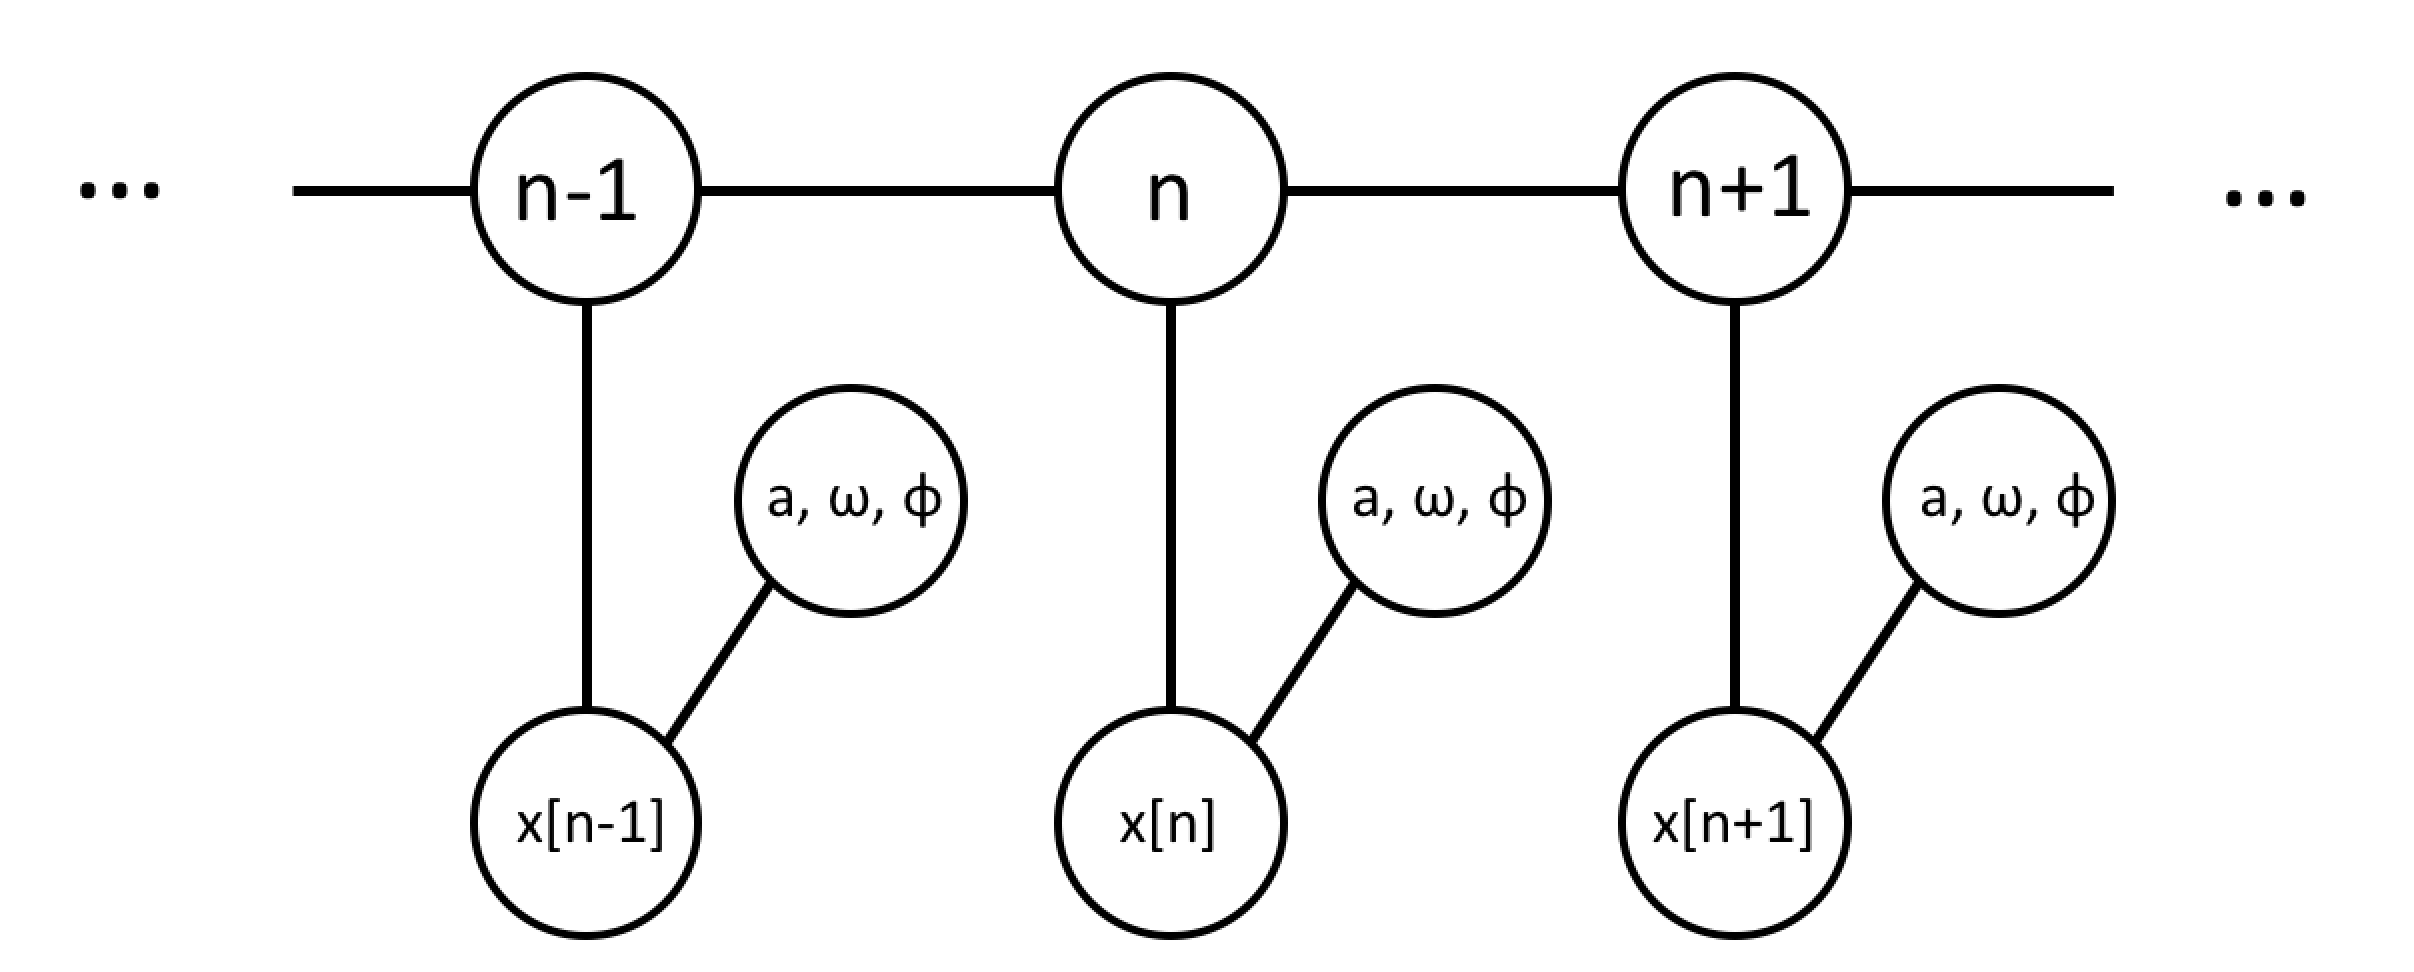
\includegraphics[width=0.5\columnwidth]{61a.png}
    \vspace{-0.1cm}
  \caption{Graphical model of 6.1(a).}
  \label{f:61a}
\end{figure}

\noindent
(b) $\s{x}_1[2n]$ is a Markov process. To show Markov property, we need to show
$p(x_1[2n] \,\big|\, x_1[2n - 2]) = p(x_1[2n] \,\big|\, x_1[2n - 2], x_1[2n -4], \cdots)$. We note that
\begin{align*}
p(x_1[2n] \,\big|\, x_1[2n - 2])	 &=
\sum_{x_1[2n - 1]} p(x_1[2n], x_1[2n-1] \,\big|\, x_1[2n - 2])\\
&= \sum_{x_1[2n - 1]} p(x_1[2n] \,\big|\, x_1[2n-1], x_1[2n-2])
p(x_1[2n-1] \,\big|\, x_1[2n-2])\\
&= \sum_{x_1[2n - 1]} p(x_1[2n] \,\big|\, x_1[2n-1], x_1[2n-2], \cdots)
p(x_1[2n-1] \,\big|\, x_1[2n-2], \cdots)\\
&\;\;\;\;\text{(since $\s{x}_1[0], \s{x}_1[1], \cdots, \s{x}_1[2n-1], \s{x}_1[2n]$ is a Markov process)}\\
&= \sum_{x_1[2n - 1]} p(x_1[2n] \,\big|\, x_1[2n-1], x_1[2n-2], x_1[2n-4], x_1[2n-6], \cdots)\\
&\;\;\;\; \times p(x_1[2n-1] \,\big|\, x_1[2n-2], x_1[2n-4], x_1[2n-6], \cdots)\\
&= \sum_{x_1[2n - 1]} p(x_1[2n], x_1[2n-1] \,\big|\, x_1[2n-2], x_1[2n-4], x_1[2n-6], \cdots)\\
& = p(x_1[2n] \,\big|\, x_1[2n-2], x_1[2n-4], x_1[2n-6], \cdots)
\end{align*} \qeds

$\s{y}[n]$ is not a Markov process. This is because $\s{y}[2n]$ is a function of
$\s{y}[2n-2]$ by construction from $\s{x}_1$. Since $\s{y}[2n]$ is independent of
$\s{y}[2n-1]$, $\s{y}[2n]$ would not be conditional independent of $\s{y}[2n-2]$ on
$\s{y}[2n-1]$. As a concrete example, let the initial state
$\s{x}[0] \sim \text{Bern}(1/2)$,
$\s{y}[0] \sim \text{Bern}(1/2)$ and the Markov process be
$\s{x}[0] = \s{x}[1] = \cdots = \s{x}[n]$, 
$\s{y}[0] = \s{y}[1] = \cdots = \s{y}[n]$. Then
\begin{align*}
	p(y[2n] \,\big|\, y[2n - 1]) = \frac{1}{2}
	\neq \mathds{1}_{y[2n] = y[2n - 2]} = p(y[2n] \,\big|\, y[2n - 1], y[2n - 2]).
\end{align*} \qeds
\pagebreak

%%%%%%%%%%%%%%%%%%%%%%%%%%%%%%%%%%%%%%%%%%%%%%%%%%%%%%%%%%%%%%%%%%%%%%%% 
\section*{Problem 6.2}
(a) First we compute
$p_{\s{x}_i | \s{x}_{\mathscr{V}\backslash i}}(\,\cdot \,| x_{\mathscr{V}\backslash \{i\}})$,
%
\begin{align}
	p_{\s{x}_i | \s{x}_{\mathscr{V}\backslash\{i\}}}(x_i| x_{\mathscr{V}\backslash \{i\}}) =
	\frac{\exp\left\{\sum_{j \in \partial i}\theta x_i x_j\right\}}
	{\exp\left\{\sum_{j \in \partial i}\theta x_j\right\} +
	\exp\left\{\sum_{j \in \partial i} -\theta x_j\right\}}. \label{eq:gibbs_node_sampler_prob}
\end{align}
Hence, for update step $t = 0, 1, \cdots$, the update rules for a node-by-node Gibbs sampler is
\begin{enumerate}
	\item Select $i \in \mathscr{V}$ from the graph $\mathscr{G}$ uniformly at random.
	\item Set $x^{t+1}_{\mathscr{V}\backslash\{i\}} = x^t_{\mathscr{V}\backslash\{i\}}$
	unchanged for all nodes other than $i$; and sample $x^{t+1}_i$ following the
	distribution $p_{\s{x}_i | \s{x}_{\mathscr{V}\backslash \{i\}}}
	(\,\cdot \,| x^t_{\mathscr{V}\backslash \{i\}})$ derived above.\\
\end{enumerate}

\noindent
(b) To generate $\bs{y} = (\s{y}_1, \s{y}_2, \cdots, \s{y}_n)$, we note that
\begin{align*}
	p(y_1, y_2, \cdots, y_n) = p(y_1)\, p (y_2 | y_1)\, p(y_3 | y_1, y_2) \cdots p(y_n | y_1, y_2, \cdots, y_{n-1}).
\end{align*}
%
\begin{figure}[h!]
  \centering
  \vspace{-0.3cm}
  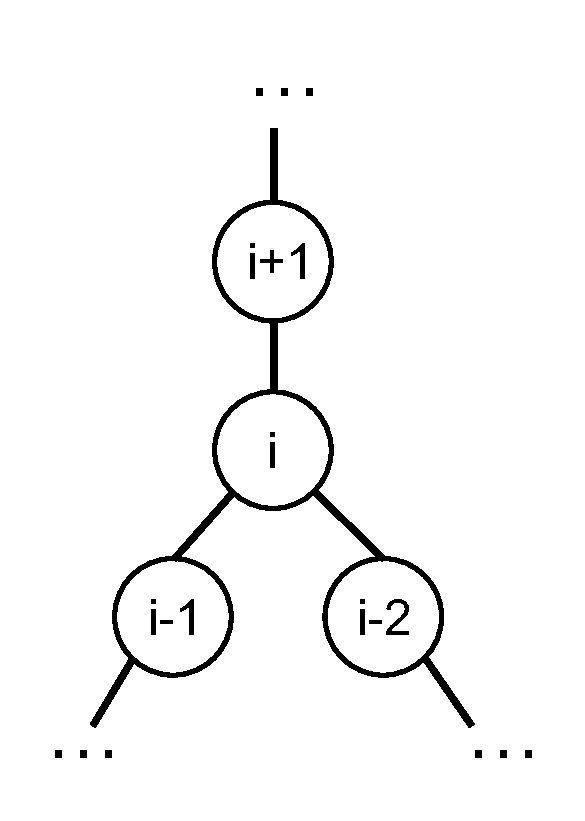
\includegraphics[width=0.2\columnwidth]{62b.pdf}
    \vspace{-0.1cm}
  \caption{Tree structured graph for problem 6.2(b).}
  \label{f:62b}
\end{figure}
%

Importantly, with a tree structure shown in Figure~\ref{f:62b}, the conditional
distribution can be determined by the samples of
$\s{y}_{i-1}, \s{y}_{i-2}, \cdots, \s{y}_{0}$, and the message passed from $\s{y}_{i+1}$
in belief propagation. Specifically\footnote{In general, we need messages from all the parent node of $i$ in the tree.},
%
\begin{align*}
	p(y_i \,\big|\, y_{i-1}, y_{i-2}, \cdots) &= \frac{p(y_i, y_{i-1}, y_{i-2}, \cdots)}{p(y_{i-1}, y_{i-2}, \cdots)}\\
	&=\frac{\sum_{y_{i+1}, y_{i+2}, \cdots} \prod_{k, l \in \mathscr{E}} \psi_{kl}(y_k, y_l)\prod_{j\in\mathscr{V}}\phi_j(y_j)}
	{\sum_{y_{i+1}, y_{i+2}, \cdots}\sum_{y_{i}}\prod_{k, l \in \mathscr{E}}\psi_{kl}(y_k, y_l)\prod_{j\in\mathscr{V}}\phi_j(y_j)} \\ 
	&= \frac{m_{i+1\to i}(y_i) \psi_{i-1, i}(y_{i-1}, y_i)\psi_{i-2, i}(y_{i-2}, y_i)\phi_i(y_i)}{\sum_{y_{i}}m_{i+1\to i}(y_i) \psi_{i-1, i}(y_{i-1}, y_i)\psi_{i-2, i}(y_{i-2}, y_i)\phi_i(y_i)}.
\end{align*}
%

In general, the conditional distribution for a node can be expressed as
\begin{align}
	p(y_i \,\big|\, y_{i-1}, y_{i-2}, \cdots) = \frac{\prod_{k \in \text{parent}(i)}m_{k\to i}(y_i)\prod_{j \in \text{children}(i)}\psi_{ij}(y_i, y_j)\phi_i(y_i)}{\sum_{y_{i}}\prod_{k \in \text{parent}(i)}m_{k\to i}(y_i)\prod_{j \in \text{children}(i)}\psi_{ij}(y_i, y_j)\phi_i(y_i)} \label{eq:62_conditional_dist}
\end{align}

Thus, we can label the nodes in the tree and sample the variables in a sequence.
%
Operationally, the efficient procedure is
\begin{enumerate}
	\item Pick a leaf node and label it as $\s{y}_1$. Set the current node index $i=1$.
	\item Run the message passing scheme\footnote{In the question, we select a root node
		  first and only aggregates the message up to that node
		  (instead of passing messages back from the root for every node).
		  For the remaining, we
		  only need the computed message to perform ``belief propagation'' for sampling.
		  Overall, each node is visited no more than twice. Hence it is still valid to say 		  ``by running belief propagation once''.}
		  to obtain the marginal distribution of $p_{\s{y}_1}(y_1)$.
	\item Sample $y_1 \sim p_{\s{y}_1}(y_1)$.
	\item For any node with all its children node labeled, label it as $\s{y}_{i+1}$.
	\item Sample $y_{i+1} \sim p(y_{i+1} \,\big|\, y_i, y_{i-1}, \cdots )$ using
		  Equation~\eqref{eq:62_conditional_dist}. Notice that at this step, the values of
		  $\s{y}_{\text{children}(i)}$ are sampled in previous steps and the messages
		  $m_{\text{parent}(i)\to i}$ are available from the belief propagation in step 2.
		  Set current node index as $i + 1$.
	\item Repeat step 4 and 5 until an instance of $\bs{y} = (\s{y}_1, \s{y}_2, \cdots, 		  \s{y}_n)$ is sampled.\\
\end{enumerate}
%

\noindent
(c) Without loss of generality, to sample $p_{\s{x}_A | \s{x}_B}$, we need to first
update the node potential (can then be absorbed in the edge potential) of
$\s{x}_A$ based on the sampled values in $\s{x}_B$. Specifically, the node potential
of a node $i$ in $\s{x}_A$ becomes
\begin{align*}
	\exp\left\{{\sum_{j \in \partial i \cap B} \theta}x_ix_j\right\}.
\end{align*}

Then we use the the sampler developed in part (b) to sample the value in the
tree structure, with the edge potential updated by the first step.

We repeat the above process and alternate between $A$ and $B$ to perform
block Gibbs sampling.
\pagebreak

%%%%%%%%%%%%%%%%%%%%%%%%%%%%%%%%%%%%%%%%%%%%%%%%%%%%%%%%%%%%%%%%%%%%%%%% 
\section*{Problem 6.3}
%
\textbf{Key routines in the program.}
%
\noindent
For Gibbs node-by-node sampler, the key routines are 
\begin{enumerate}
	\item Initialization of node values (e.g., all $+1$ or all $-1$). Initialization of edge potentials. (Figure~\ref{f:code}a)
	\item In each iteration on a node, compute the probability of choosing $+1$, based on edge potential
	  	  and the values of the neighbor nodes. The probability is computed
	  	  in Equation~\eqref{eq:gibbs_node_sampler_prob} from Problem 6.2. (Figure~\ref{f:code}b)
	\item A loop through all nodes in each sampling iteration. (Figure~\ref{f:code}c)
\end{enumerate}
%
For Gibbs comb block sampler, the key routines are
\begin{enumerate}
	\item Initialization of node values (e.g., all $+1$ or all $-1$). Initialization of edge potentials. This
	      step is the same as Gibbs node-by-node sampler. (Figure~\ref{f:code}a)
	\item A message update routine to aggregate messages for specified destination (requiring source message all aggregated). 
	      (Figure~\ref{f:code}d)
	\item A serial belief propagation routine that calls the message update following a traversal order
	      (from the proper indexing in Problem 6.2(b)). (Figure~\ref{f:code}e)
	\item A scheme to determine the tree traversal order (indexing) for the two combs. (Figure~\ref{f:code}f)
	\item In each iteration on a node, update the node and edge potential in the tree path, and then
	      perform serial belief propagation to get all the messages on one direction.
	      Start sampling from the marginals. Based on the sampled value and passed messages,
	      sample the conditional probability using Equation~\eqref{eq:62_conditional_dist} from Problem 6.2(b). (Figure~\ref{f:code}g)
	\item A loop through all nodes in each sampling iteration. (Figure~\ref{f:code}h)
\end{enumerate}

\noindent
\textbf{Visualization of the samples.}
\noindent
We run the Gibbs node-by-node and the comb-shaped block sampler for 1000 iterations, initializing the nodes by
all $+1$ or all $-1$. The samples are visualized in Figure~\ref{f:63a}.
%
\begin{figure*}[h]
\captionsetup[subfigure]{labelformat=empty}
\centering
%
\begin{subfigure}[t]{0.09\textwidth}
\centering

\includegraphics[width=\textwidth]{./computational/results/gibbs_node_sampler_positive_iter_0.png}
\vspace{-0.6cm}
\end{subfigure}\hspace{0.001\textwidth}
%
%
\begin{subfigure}[t]{0.09\textwidth}
\centering

\includegraphics[width=\textwidth]{./computational/results/gibbs_node_sampler_positive_iter_100.png}
\vspace{-0.6cm}
\end{subfigure}\hspace{0.001\textwidth}
%
%
\begin{subfigure}[t]{0.09\textwidth}
\centering

\includegraphics[width=\textwidth]{./computational/results/gibbs_node_sampler_positive_iter_200.png}
\vspace{-0.6cm}
\end{subfigure}\hspace{0.001\textwidth}
%
%
\begin{subfigure}[t]{0.09\textwidth}
\centering

\includegraphics[width=\textwidth]{./computational/results/gibbs_node_sampler_positive_iter_300.png}
\vspace{-0.6cm}
\end{subfigure}\hspace{0.001\textwidth}
%
%
\begin{subfigure}[t]{0.09\textwidth}
\centering

\includegraphics[width=\textwidth]{./computational/results/gibbs_node_sampler_positive_iter_400.png}
\vspace{-0.6cm}
\end{subfigure}\hspace{0.001\textwidth}
%
%
\begin{subfigure}[t]{0.09\textwidth}
\centering

\includegraphics[width=\textwidth]{./computational/results/gibbs_node_sampler_positive_iter_500.png}
\vspace{-0.6cm}
\end{subfigure}\hspace{0.001\textwidth}
%
%
\begin{subfigure}[t]{0.09\textwidth}
\centering

\includegraphics[width=\textwidth]{./computational/results/gibbs_node_sampler_positive_iter_600.png}
\vspace{-0.6cm}
\end{subfigure}\hspace{0.001\textwidth}
%
%
\begin{subfigure}[t]{0.09\textwidth}
\centering

\includegraphics[width=\textwidth]{./computational/results/gibbs_node_sampler_positive_iter_700.png}
\vspace{-0.6cm}
\end{subfigure}\hspace{0.001\textwidth}
%
%
\begin{subfigure}[t]{0.09\textwidth}
\centering

\includegraphics[width=\textwidth]{./computational/results/gibbs_node_sampler_positive_iter_800.png}
\vspace{-0.6cm}
\end{subfigure}\hspace{0.001\textwidth}
%
%
\begin{subfigure}[t]{0.09\textwidth}
\centering

\includegraphics[width=\textwidth]{./computational/results/gibbs_node_sampler_positive_iter_900.png}
\vspace{-0.6cm}
\end{subfigure}\hspace{0.001\textwidth}
%
%
\begin{subfigure}[t]{0.09\textwidth}
\centering

\includegraphics[width=\textwidth]{./computational/results/gibbs_node_sampler_negative_iter_0.png}
\vspace{-0.6cm}
\end{subfigure}\hspace{0.001\textwidth}
%
%
\begin{subfigure}[t]{0.09\textwidth}
\centering

\includegraphics[width=\textwidth]{./computational/results/gibbs_node_sampler_negative_iter_100.png}
\vspace{-0.6cm}
\end{subfigure}\hspace{0.001\textwidth}
%
%
\begin{subfigure}[t]{0.09\textwidth}
\centering

\includegraphics[width=\textwidth]{./computational/results/gibbs_node_sampler_negative_iter_200.png}
\vspace{-0.6cm}
\end{subfigure}\hspace{0.001\textwidth}
%
%
\begin{subfigure}[t]{0.09\textwidth}
\centering

\includegraphics[width=\textwidth]{./computational/results/gibbs_node_sampler_negative_iter_300.png}
\vspace{-0.6cm}
\end{subfigure}\hspace{0.001\textwidth}
%
%
\begin{subfigure}[t]{0.09\textwidth}
\centering

\includegraphics[width=\textwidth]{./computational/results/gibbs_node_sampler_negative_iter_400.png}
\vspace{-0.6cm}
\end{subfigure}\hspace{0.001\textwidth}
%
%
\begin{subfigure}[t]{0.09\textwidth}
\centering

\includegraphics[width=\textwidth]{./computational/results/gibbs_node_sampler_negative_iter_500.png}
\vspace{-0.6cm}
\end{subfigure}\hspace{0.001\textwidth}
%
%
\begin{subfigure}[t]{0.09\textwidth}
\centering

\includegraphics[width=\textwidth]{./computational/results/gibbs_node_sampler_negative_iter_600.png}
\vspace{-0.6cm}
\end{subfigure}\hspace{0.001\textwidth}
%
%
\begin{subfigure}[t]{0.09\textwidth}
\centering

\includegraphics[width=\textwidth]{./computational/results/gibbs_node_sampler_negative_iter_700.png}
\vspace{-0.6cm}
\end{subfigure}\hspace{0.001\textwidth}
%
%
\begin{subfigure}[t]{0.09\textwidth}
\centering

\includegraphics[width=\textwidth]{./computational/results/gibbs_node_sampler_negative_iter_800.png}
\vspace{-0.6cm}
\end{subfigure}\hspace{0.001\textwidth}
%
%
\begin{subfigure}[t]{0.09\textwidth}
\centering

\includegraphics[width=\textwidth]{./computational/results/gibbs_node_sampler_negative_iter_900.png}
\vspace{-0.6cm}
\end{subfigure}\hspace{0.001\textwidth}
%
%
\begin{subfigure}[t]{0.09\textwidth}
\centering

\includegraphics[width=\textwidth]{./computational/results/gibbs_comb_sampler_positive_iter_0.png}
\vspace{-0.6cm}
\end{subfigure}\hspace{0.001\textwidth}
%
%
\begin{subfigure}[t]{0.09\textwidth}
\centering

\includegraphics[width=\textwidth]{./computational/results/gibbs_comb_sampler_positive_iter_100.png}
\vspace{-0.6cm}
\end{subfigure}\hspace{0.001\textwidth}
%
%
\begin{subfigure}[t]{0.09\textwidth}
\centering

\includegraphics[width=\textwidth]{./computational/results/gibbs_comb_sampler_positive_iter_200.png}
\vspace{-0.6cm}
\end{subfigure}\hspace{0.001\textwidth}
%
%
\begin{subfigure}[t]{0.09\textwidth}
\centering

\includegraphics[width=\textwidth]{./computational/results/gibbs_comb_sampler_positive_iter_300.png}
\vspace{-0.6cm}
\end{subfigure}\hspace{0.001\textwidth}
%
%
\begin{subfigure}[t]{0.09\textwidth}
\centering

\includegraphics[width=\textwidth]{./computational/results/gibbs_comb_sampler_positive_iter_400.png}
\vspace{-0.6cm}
\end{subfigure}\hspace{0.001\textwidth}
%
%
\begin{subfigure}[t]{0.09\textwidth}
\centering

\includegraphics[width=\textwidth]{./computational/results/gibbs_comb_sampler_positive_iter_500.png}
\vspace{-0.6cm}
\end{subfigure}\hspace{0.001\textwidth}
%
%
\begin{subfigure}[t]{0.09\textwidth}
\centering

\includegraphics[width=\textwidth]{./computational/results/gibbs_comb_sampler_positive_iter_600.png}
\vspace{-0.6cm}
\end{subfigure}\hspace{0.001\textwidth}
%
%
\begin{subfigure}[t]{0.09\textwidth}
\centering

\includegraphics[width=\textwidth]{./computational/results/gibbs_comb_sampler_positive_iter_700.png}
\vspace{-0.6cm}
\end{subfigure}\hspace{0.001\textwidth}
%
%
\begin{subfigure}[t]{0.09\textwidth}
\centering

\includegraphics[width=\textwidth]{./computational/results/gibbs_comb_sampler_positive_iter_800.png}
\vspace{-0.6cm}
\end{subfigure}\hspace{0.001\textwidth}
%
%
\begin{subfigure}[t]{0.09\textwidth}
\centering

\includegraphics[width=\textwidth]{./computational/results/gibbs_comb_sampler_positive_iter_900.png}
\vspace{-0.6cm}
\end{subfigure}\hspace{0.001\textwidth}
%
%
\begin{subfigure}[t]{0.09\textwidth}
\centering

\includegraphics[width=\textwidth]{./computational/results/gibbs_comb_sampler_negative_iter_0.png}
\vspace{-0.6cm}
\end{subfigure}\hspace{0.001\textwidth}
%
%
\begin{subfigure}[t]{0.09\textwidth}
\centering

\includegraphics[width=\textwidth]{./computational/results/gibbs_comb_sampler_negative_iter_100.png}
\vspace{-0.6cm}
\end{subfigure}\hspace{0.001\textwidth}
%
%
\begin{subfigure}[t]{0.09\textwidth}
\centering

\includegraphics[width=\textwidth]{./computational/results/gibbs_comb_sampler_negative_iter_200.png}
\vspace{-0.6cm}
\end{subfigure}\hspace{0.001\textwidth}
%
%
\begin{subfigure}[t]{0.09\textwidth}
\centering

\includegraphics[width=\textwidth]{./computational/results/gibbs_comb_sampler_negative_iter_300.png}
\vspace{-0.6cm}
\end{subfigure}\hspace{0.001\textwidth}
%
%
\begin{subfigure}[t]{0.09\textwidth}
\centering

\includegraphics[width=\textwidth]{./computational/results/gibbs_comb_sampler_negative_iter_400.png}
\vspace{-0.6cm}
\end{subfigure}\hspace{0.001\textwidth}
%
%
\begin{subfigure}[t]{0.09\textwidth}
\centering

\includegraphics[width=\textwidth]{./computational/results/gibbs_comb_sampler_negative_iter_500.png}
\vspace{-0.6cm}
\end{subfigure}\hspace{0.001\textwidth}
%
%
\begin{subfigure}[t]{0.09\textwidth}
\centering

\includegraphics[width=\textwidth]{./computational/results/gibbs_comb_sampler_negative_iter_600.png}
\vspace{-0.6cm}
\end{subfigure}\hspace{0.001\textwidth}
%
%
\begin{subfigure}[t]{0.09\textwidth}
\centering

\includegraphics[width=\textwidth]{./computational/results/gibbs_comb_sampler_negative_iter_700.png}
\vspace{-0.6cm}
\end{subfigure}\hspace{0.001\textwidth}
%
%
\begin{subfigure}[t]{0.09\textwidth}
\centering

\includegraphics[width=\textwidth]{./computational/results/gibbs_comb_sampler_negative_iter_800.png}
\vspace{-0.6cm}
\end{subfigure}\hspace{0.001\textwidth}
%
%
\begin{subfigure}[t]{0.09\textwidth}
\centering

\includegraphics[width=\textwidth]{./computational/results/gibbs_comb_sampler_negative_iter_900.png}
\vspace{-0.6cm}
\end{subfigure}\hspace{0.001\textwidth}
%
\caption{Visualization of the Gibbs samples.
         1st row: node-by-node samples, initialized with all $+1$.
         2nd row: node-by-node samples, initialized with all $-1$.
         3rd row: block samples, initialized with all $+1$.
         4th row: block samples, initialized with all $-1$.
         Each column corresponds to $\{1, 100, 200, \cdots, 900\}$ iterations.
         The $+1$ region is denoted as white, $-1$ as black.}
\label{f:63a}
\end{figure*}
%

\noindent
\textbf{Analysis.}
\noindent
By symmetry, there should not be a bias between $+1$ or $-1$ samples.
%
Thus, over a long time, the samples should give $+1$ or $-1$ with the same probability for all nodes.
%
However, since $\theta=0.45$ is relatively large, the values of the nodes tend to stick with each
other; and the mixing time can be long.
%
We plot the average value of all nodes over $20,000$ Markov process steps for both sampler in Figure~\ref{f:63}.
%
From the figure, Gibbs block sampler oscillates between the $+1$ and $-1$ regions more often;
and the mixing time should be empirically shorter. 
%

In terms of per-sweep running time, the complexity is both $O(n)$. Since the block sampling scheme has
an extra step for message passing and updating the node potentials from the observation of the other block,
the empirical runtime for the block sampler is slightly longer ($\sim 2\times$ longer in my implementation).

Also from figure~\ref{f:63}, different initializations affect which $+1/-1$ region to sample first the
but don't empirically affect the mixing time.
\\

\begin{figure*}[h]
\centering
\vspace{-0.6cm}
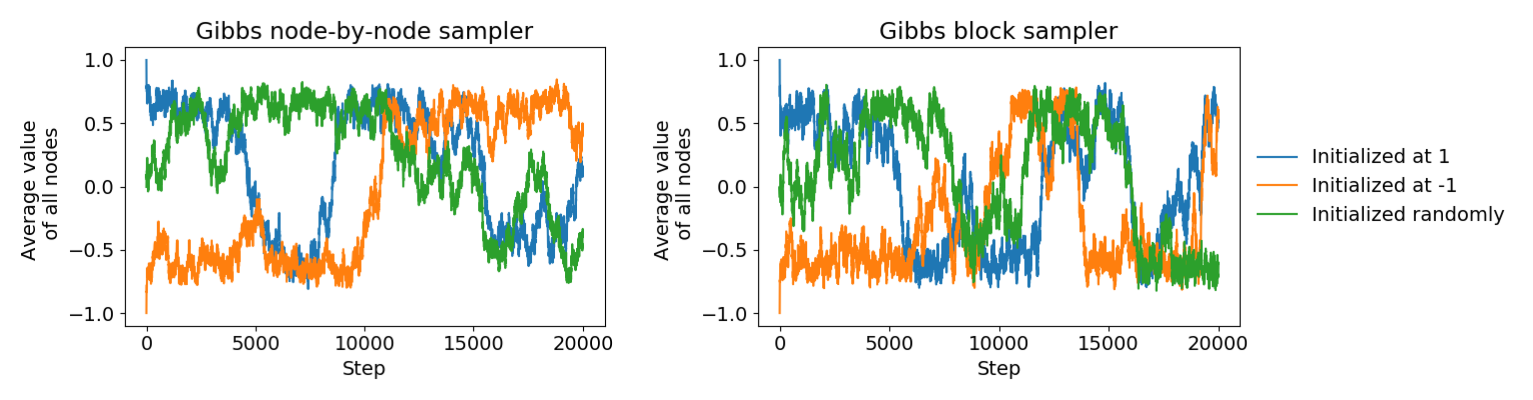
\includegraphics[width=\textwidth]{./63.pdf}
\vspace{-0.8cm}
\caption{Mixing behavior of Gibbs samplers. Left: node-by-node sampler. Right: comb-shaped block sampler.}
\label{f:63}
\end{figure*}

\noindent
\textbf{Code snippets.}
The code snippets are included in Figure~\ref{f:code}.
%
\begin{figure*}[h]
\centering
\vspace{-0.2cm}
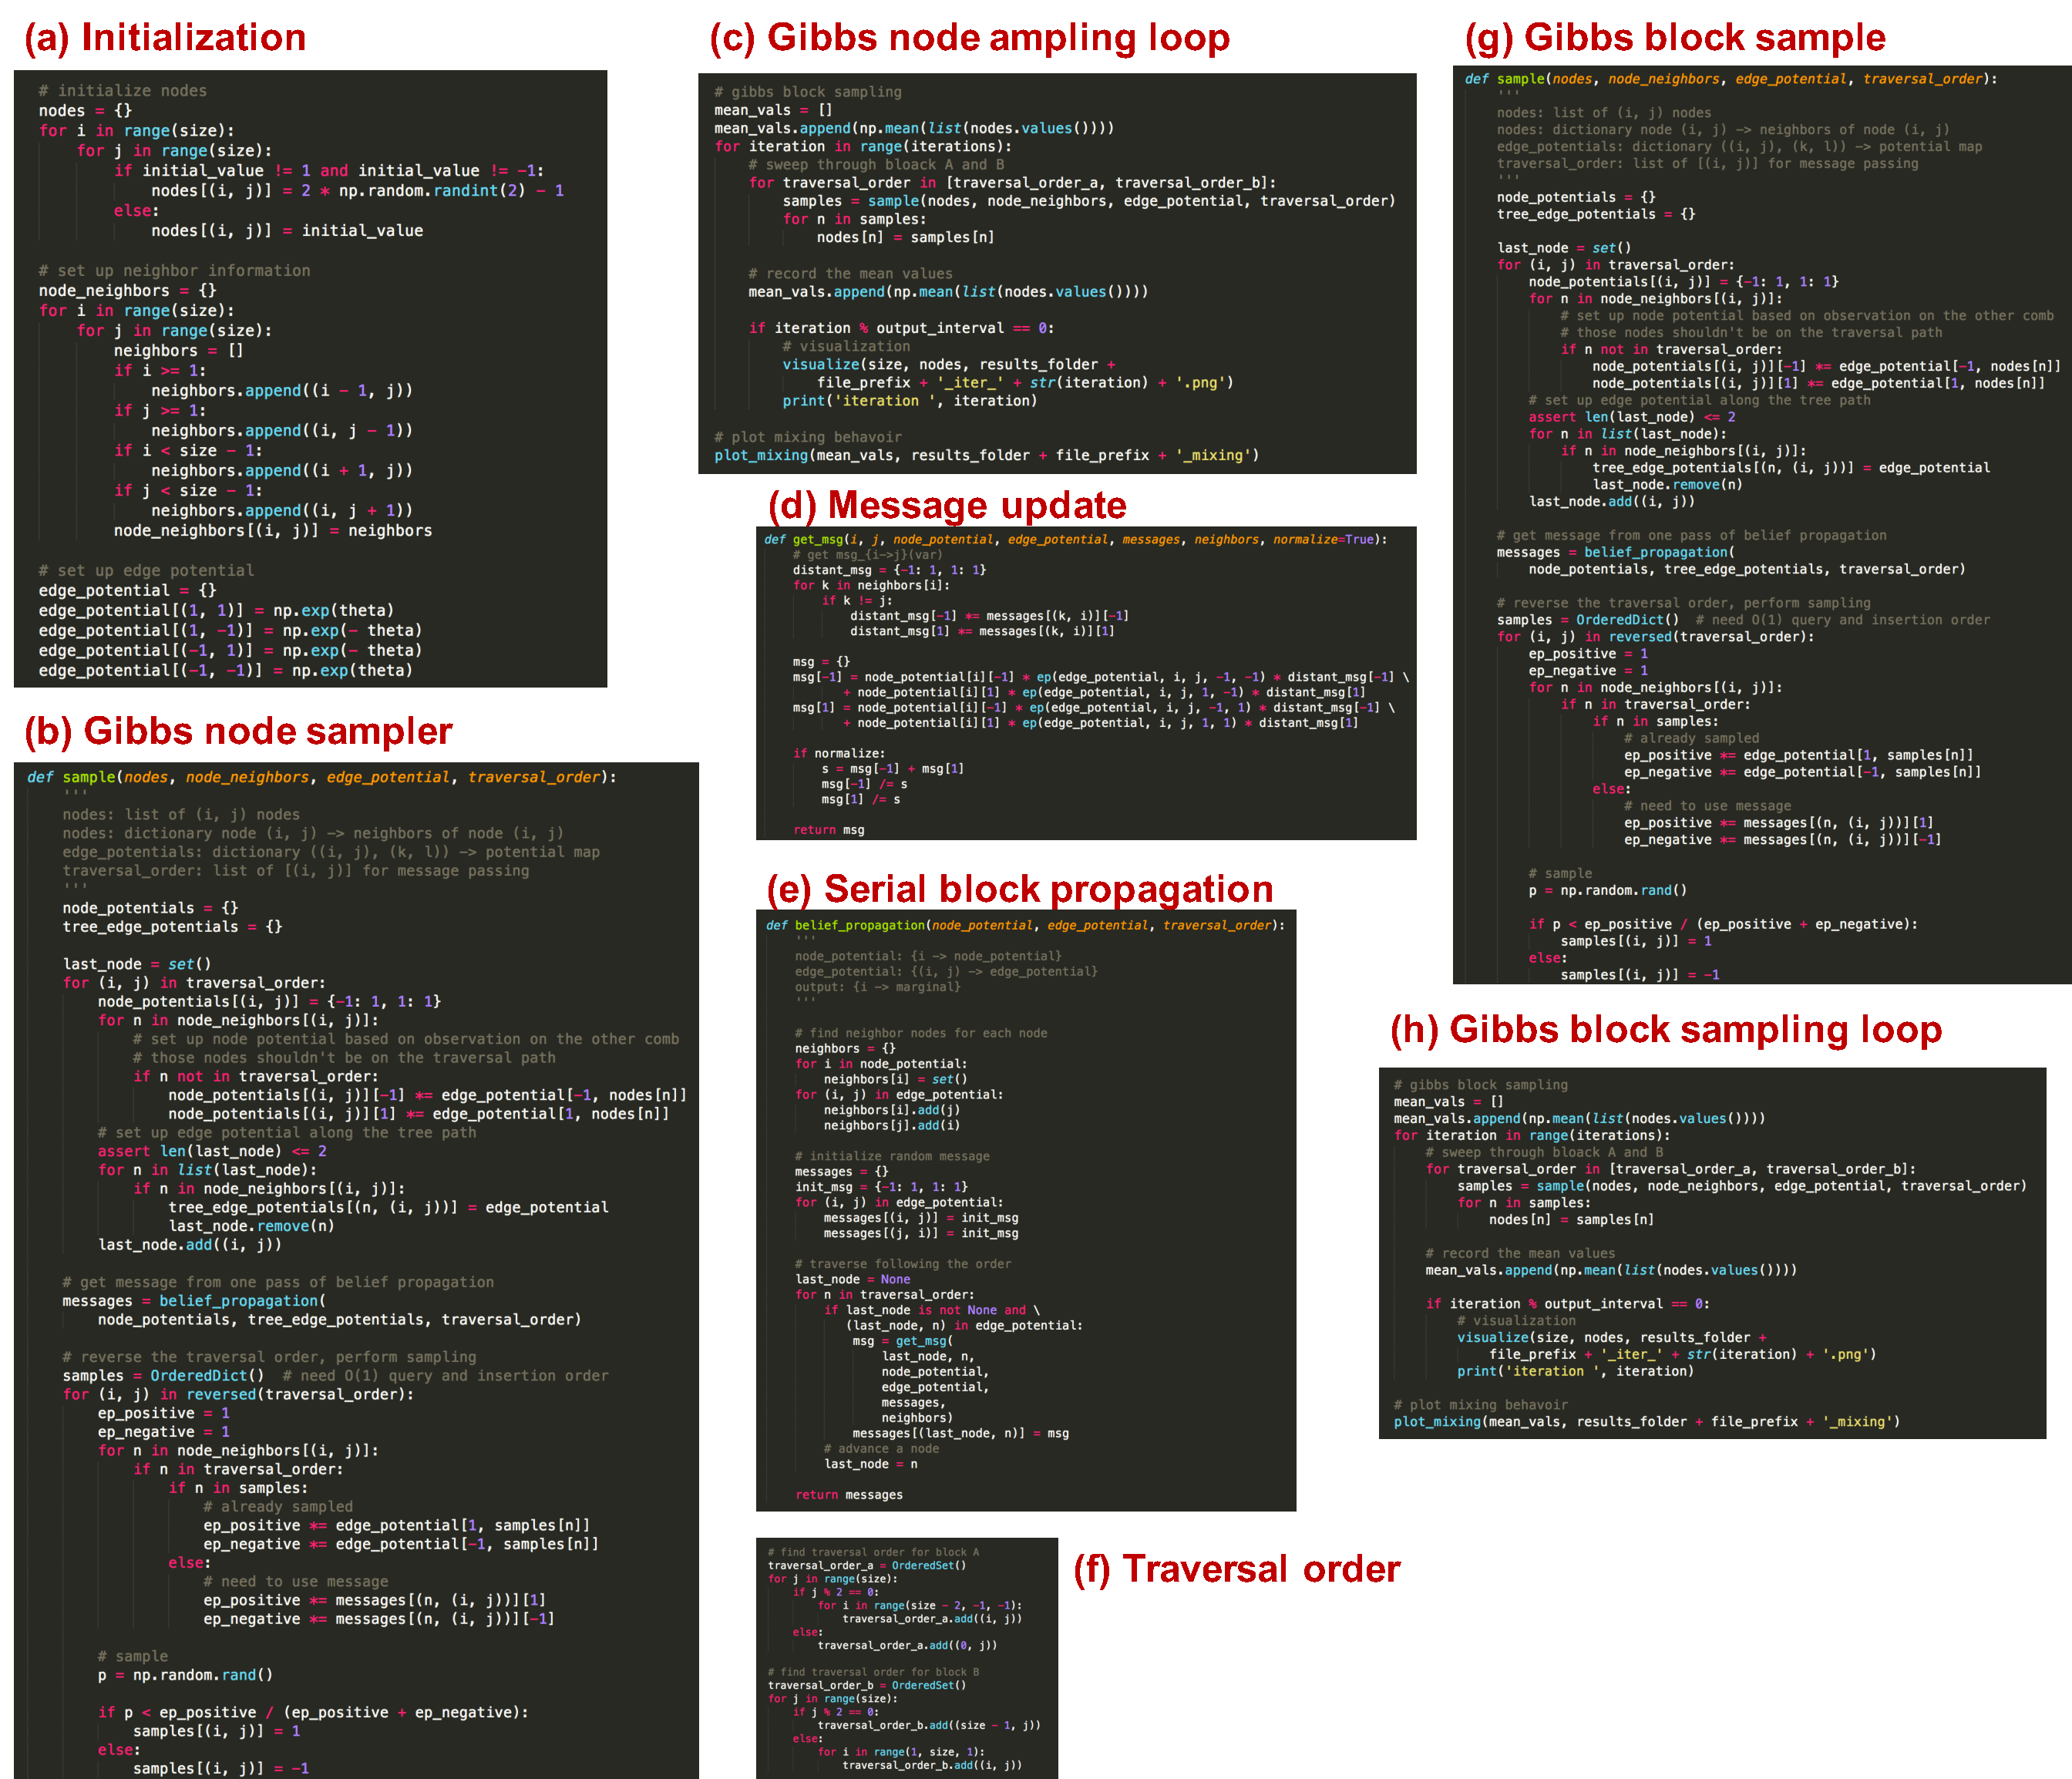
\includegraphics[width=0.98\textwidth]{./computational/code_screenshots/code.pdf}
\vspace{-0.2cm}
\caption{Code snippets for Gibbs sampler.}
\label{f:code}
\end{figure*}

\pagebreak
%%%%%%%%%%%%%%%%%%%%%%%%%%%%%%%%%%%%%%%%%%%%%%%%%%%%%%%%%%%%%%%%%%%%%%%% 
\section*{Problem 6.4}
(a) Since every matching has the same probability (i.e., $w_{ij} = 0$), we can repeat
the following process until a matching is formed
\begin{enumerate}
	\item randomly pick a node $i$ from $v$;
	\item randomly pick a node $j$ from $u$, which establishes $\sigma_{ij}=1$;
	\item remove $i$ from $v$ and remove $j$ from $u$.\\
\end{enumerate}

\noindent
(b) We note that
\begin{align}
	Z &= \sum_{\sigma\in\text{ perfect matchings}} \exp\left(\sum_{i,j}w_{ij}\sigma_{ij}\right)\\
	&\leq \sum_{\sigma\in\text{ perfect matchings}} \exp\left(Nw^*\right) \label{eq:64b_1}\\
	&\leq N!\exp\left(Nw^*\right) \label{eq:64b_2}.
\end{align}

Here, \eqref{eq:64b_1} is because for perfect matching,
$\sum_{k=1}^N \sigma_{ik} = 1$, for all $1\leq i \leq N$; and
$\sum_{k=1}^N \sigma_{kj} = 1$, for all $1\leq j \leq N$.
Inequality \eqref{eq:64b_2} is because there are $N!$ possible
distinct perfect matchings. This is because for the first node in $v$,
there is $N$ possible destination node to match in $u$;
after the first node occupies a node in $u$, the second node in $v$ has $N-1$ nodes
left in $u$;
the third node in $v$ then has $N-2$ nodes in $u$ and so on.

Then we have for any perfect matching $\sigma$
\begin{align}
	p(\sigma) &= \frac{\exp\left(\sum_{i,j}w_{ij}\sigma_{ij}\right)\mathds{1}_{\sigma \text{ is perfect matching}}}{Z}\\
	& \geq \frac{1}{Z} \label{eq:64b_3}\\
	& \geq \frac{1}{N!\exp\left(Nw^*\right)}, \label{eq:64b_4}
\end{align}
where \eqref{eq:64b_3} is because $w_{ij} \geq 0$, $\sigma_{ij} \geq 0$, $\mathds{1}_{\sigma \text{ is perfect matching}} = 1$; and \eqref{eq:64b_4} is because of \eqref{eq:64b_2}. \qeds
\\

\noindent
(c) For the defined Markov chain, we can explicitly write out the probability of valid
transition $\sigma \to \sigma'$
\begin{align}
	\bm{P}_{\sigma \sigma'} &= \frac{1}{N^2}\min(1, \exp(w_{i\sigma(j)} + w_{j\sigma(i)} - w_{i\sigma(i)} - w_{j\sigma(j)}))\label{eq:64b_5}\\
	&\geq \frac{1}{N^2}\exp(-2w^*). \label{eq:64b_6}
\end{align}
where \eqref{eq:64b_5} is because we choose $i, j \in \{1, 2, \cdots, N\}$ randomly; and 
\eqref{eq:64b_6} is because $w_{ij} \geq 0$ and $-w_{ij} \geq -w^*$. \qeds
\\

\noindent
(d) Using the results from (b) and (c), we immediately have
\begin{align*}
	p(\sigma)\bm{P}_{\sigma\sigma'} \geq \frac{1}{N!\exp\left(Nw^*\right)}\frac{1}{N^2}\exp(-2w^*),
\end{align*}
for all valid $\sigma, \sigma'$.

Now notice that in the nominator of $\Phi$, we have
\begin{align*}
	\sum_{\sigma\in S, \sigma'\in S'} p(\sigma)\bm{P}_{\sigma\sigma'} \geq \min_{\sigma, \sigma'}\bigg[ p(\sigma)\bm{P}_{\sigma\sigma'}\bigg] \geq \frac{1}{N!\exp\left(Nw^*\right)}\frac{1}{N^2}\exp(-2w^*).
\end{align*}

And in the denominator of $\Phi$, we have
\begin{align*}
p(S)p(S') \leq 1 \times 1 = 1,
\end{align*} for all valid $S, S'$.

Thus, we have
\begin{align*}
	\Phi \geq \frac{1}{N!\exp\left(Nw^*\right)}\frac{1}{N^2}\exp(-2w^*).
\end{align*}\qeds
\\

\noindent
(e) Using the results from (b) and (d), we have
\begin{align*}
	T_{mix}(\epsilon) &\leq \frac{1}{\Phi^2}\left(\log\frac{1}{\min_\sigma p (\sigma)} + \log\frac{1}{\epsilon}\right)\\
	&\leq \frac{(N!)^2 N^4 \exp(2Nw^*)}{\exp(-4w^*)}\left(\log\big[N!\exp(N w^*)\big] + \log\frac{1}{\epsilon}\right).
\end{align*}


\end{document}